\documentclass{article}

\usepackage{graphicx}
\usepackage[margin=1in]{geometry}
\usepackage{booktabs}
\usepackage{placeins}
\usepackage{float}

\begin{document}

\title{Kernel Composition Report}
\author{}
\date{6 February 2026}
\maketitle

\section*{Overview}
This report summarizes kernel composition experiments and compares them to prior runs. The goal is to evaluate whether composing more kernels improves performance and also and to visualize the resulting composite filters.

\section*{Composition configurations}
\begin{center}
\begin{tabular}{lcccc}
\toprule
Run & total number of kernels & comp. pool & Test AUC & Test ACC \\
\midrule
A & 90 & 25 & 0.8662 & 0.7968 \\
B & 450 & 125 & 0.8666 & 0.7920 \\
C & 2250 & 625 & 0.8869 & 0.8107 \\
D & 4500 & 1250 & 0.8933 & 0.8150 \\

\bottomrule
\end{tabular}
\end{center}

\section*{Kernel visualization (composite filters)}
Each image below shows the learned composite kernel (red/blue indicate positive/negative response regions). Stronger contrast suggests a more selective filter, while broader smooth regions indicate texture/low-frequency emphasis.

\begin{figure}[htbp]
    \centering
    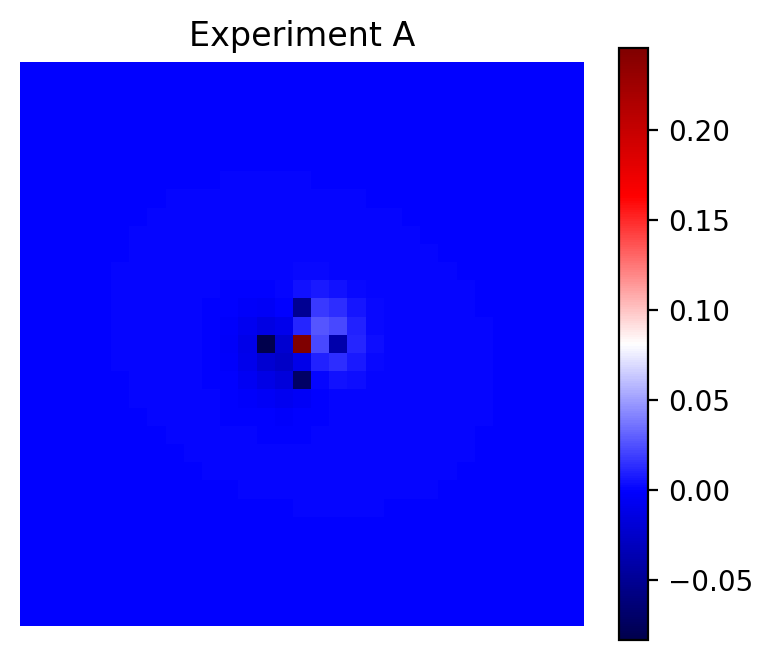
\includegraphics[width=0.24\linewidth]{../results/exp_022_mmr_nperFamily10_nComposition25/composite_kernel.png}
    \hfill
    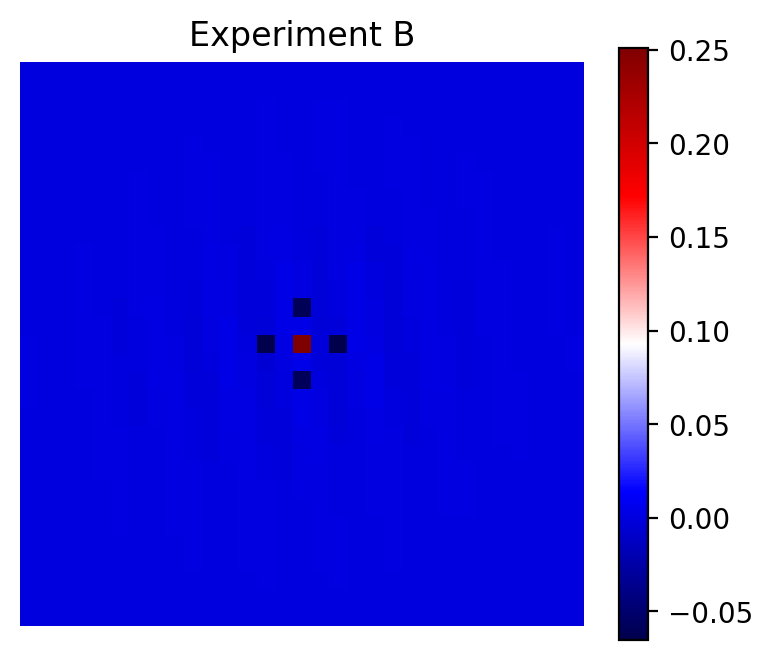
\includegraphics[width=0.24\linewidth]{../results/exp_022_mmr_nperFamily50_nComposition125/composite_kernel.png}
    \hfill
    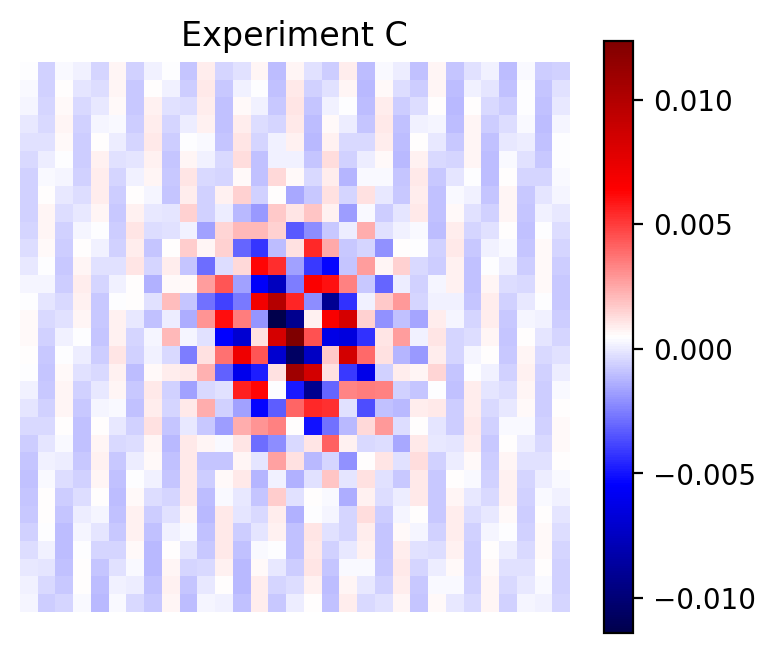
\includegraphics[width=0.24\linewidth]{../results/exp_022_mmr_nperFamily250_nComposition625/composite_kernel.png}
    \hfill
    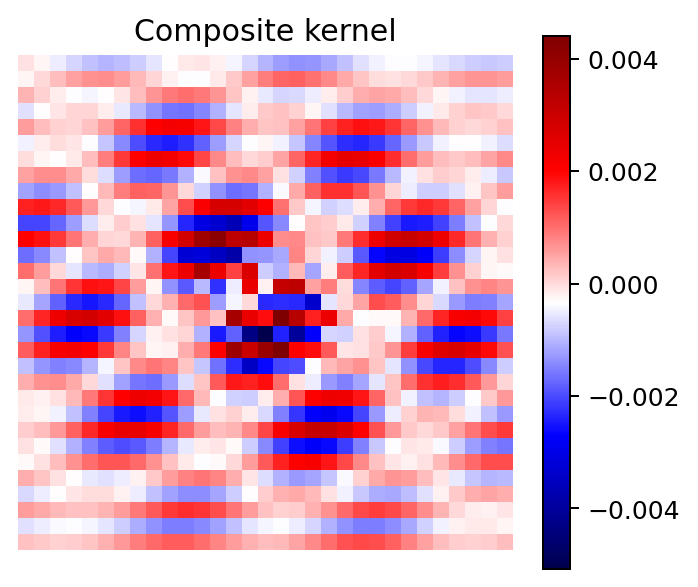
\includegraphics[width=0.24\linewidth]{../results/exp_022_mmr_nperFamily500_nComposition1250/composite_kernel.png}
    \caption{Composite kernels for A, B, C, and D (left to right).}
\end{figure}

% \section*{Heatmap examples}
% \begin{figure}[H]
%     \centering
%     
\includegraphics[width=0.95\linewidth]{../results/exp_022_mmr_nperFamily50_nComposition125/heatmaps_side_by_side.png}
%     \caption{Heatmaps for experiment with highest accuracy (87\%).}
% \end{figure}

\section*{Comparison with prior experiments}
Compared with earlier baselines (best test AUC 0.9239 from \texttt{exp\_022\_mmr} and best test ACC 0.8182 from \texttt{exp\_025\_mmr}), run D yields the strongest composite test accuracy (0.8150) and the highest composite test AUC (0.8933). ABESS runs peak at test AUC 0.9236 and ACC 0.8032, which are below the composite accuracy of run D.

\section*{How parameter changes affect quality}
\begin{itemize}
    \item Increasing the composition pool size (25 $\rightarrow$ 125 $\rightarrow$ 625 $\rightarrow$ 1250) steadily improves composite AUC/ACC.
    \item Larger total kernel banks provide more diverse filters for composition, which improves composite stability and accuracy.
    \item The largest pool (D) delivers the best composite test accuracy and AUC among composition runs.
\end{itemize}

\section*{Composition vs non-composition accuracy}
\begin{center}
\begin{tabular}{lcc}
\toprule
Run & Test ACC (regular) & Test ACC (composite) \\
\midrule
A & 0.8487 & 0.7968 \\
B & 0.8503 & 0.7920 \\
C & 0.8492 & 0.8107 \\
D & 0.8733 & 0.8150 \\
\bottomrule
\end{tabular}
\end{center}

\section*{Observation: many kernels vs single composite}
Based on the previous runs, the single composite-kernel approach is preferable. It outperforms the large multi-kernel baselines while remaining simpler, faster, and easier to deploy.

\section*{Conclusion}
Run D (500 kernels per family with a 1250-kernel composition) is the best overall. It achieves the highest composite test AUC (0.8933) and composite test accuracy (0.8150), and it also delivers the best regular-model test accuracy (0.8733). Composition improves interpretability and consistency, while the regular model maintains a higher ceiling on accuracy.

\section*{Next steps}
\begin{itemize}
    \item Run more experiments with different parameter settings to further improve accuracy.
    \item Evaluate on a new dataset to confirm generalization.
    \item Study learning a kernel-generating model to produce strong kernels without random sampling.
\end{itemize}

\end{document}
